\documentclass[a4paper,12pt]{ltjsarticle}
\usepackage{luatexja}
\usepackage{amsmath,amssymb,amsthm}
\usepackage{tikz}
\usetikzlibrary{cd,arrows,positioning}
\usepackage{mathtools}
\usepackage{listings}
\usepackage{xcolor}
\usepackage{hyperref}

\theoremstyle{definition}
\newtheorem{definition}{定義}[section]
\newtheorem{theorem}[definition]{定理}
\newtheorem{proposition}[definition]{命題}
\newtheorem{lemma}[definition]{補題}
\newtheorem{example}[definition]{例}
\newtheorem{remark}[definition]{注意}

\title{構造塔理論と離散確率論の融合\\
アルゴリズミック・マルチンゲール理論}
\author{%
  コード生成：Claude Code (Anthropic)\\
  Leanファイル生成：Codex (OpenAI)\\
  形式化日：\today
}
\date{}

\begin{document}

\maketitle

\begin{abstract}
本論文は、離散有限標本空間上の確率論を構造塔 (Structure Tower) 理論の枠組みで統一的に扱う形式化を提示する。
DecidableEvents から始まり、DecidableAlgebra、DecidableFiltration を経て、ComputableStoppingTime に至る階層構造を構築し、
最終的に Optional Stopping Theorem (OST) の計算可能版を証明する。すべての構成要素は Lean 4 で形式化され、計算可能性が保証されている。
\end{abstract}

\tableofcontents

\section{序論}

\subsection{背景と動機}

確率論の古典的な理論は、無限標本空間と $\sigma$-代数に基づいて構築されている。
しかし、計算可能性や形式検証の観点からは、有限標本空間上の離散版理論の方が取り扱いやすい。
本論文では、以下の階層構造を通じて、離散確率論の理論を構築する：

\begin{center}
\begin{tikzpicture}[node distance=2cm]
\node (DE) {DecidableEvents};
\node (DA) [below of=DE] {DecidableAlgebra};
\node (DF) [below of=DA] {DecidableFiltration};
\node (CST) [below of=DF] {ComputableStoppingTime};
\node (AMC) [below of=CST] {AlgorithmicMartingaleCore};
\node (AM) [below of=AMC] {AlgorithmicMartingale};

\draw[->] (DE) -- node[right] {事象の構造化} (DA);
\draw[->] (DA) -- node[right] {時間構造の導入} (DF);
\draw[->] (DF) -- node[right] {停止時間の定義} (CST);
\draw[->] (CST) -- node[right] {確率測度の導入} (AMC);
\draw[->] (AMC) -- node[right] {OST の証明} (AM);
\end{tikzpicture}
\end{center}

\subsection{構造塔理論との接続}

構造塔 (Structure Tower) とは、以下のデータからなる代数的構造である：

\begin{definition}[構造塔]
構造塔 $\mathcal{T}$ は以下のデータからなる：
\begin{itemize}
\item 台集合 $X$ (carrier)
\item 指標集合 $I$ (Index) と順序 $\leq$
\item 層関数 $\text{layer} : I \to \mathcal{P}(X)$
\item 被覆性：$\forall x \in X, \exists i \in I, x \in \text{layer}(i)$
\item 単調性：$i \leq j \Rightarrow \text{layer}(i) \subseteq \text{layer}(j)$
\item 最小層関数 $\text{minLayer} : X \to I$
\item 健全性：$\forall x, x \in \text{layer}(\text{minLayer}(x))$
\item 最小性：$\forall x, i, x \in \text{layer}(i) \Rightarrow \text{minLayer}(x) \leq i$
\end{itemize}
\end{definition}

本論文の主張は、DecidableFiltration が構造塔の自然なインスタンスになることである。

\section{DecidableStructureTower\_Examples：構造塔の具体例}

構造塔理論の具体的な理解のため、計算可能な例を提示する。

\subsection{整数塔：絶対値による階層化}

\begin{definition}[整数の絶対値塔]
整数 $\mathbb{Z}$ 上の構造塔 \texttt{intAbsTower} を次のように定義する：
\begin{itemize}
\item $\text{carrier} = \mathbb{Z}$
\item $\text{Index} = \mathbb{N}$
\item $\text{layer}(n) = \{k \in \mathbb{Z} \mid |k| \leq n\}$
\item $\text{minLayer}(k) = |k|$
\end{itemize}
\end{definition}

\begin{center}
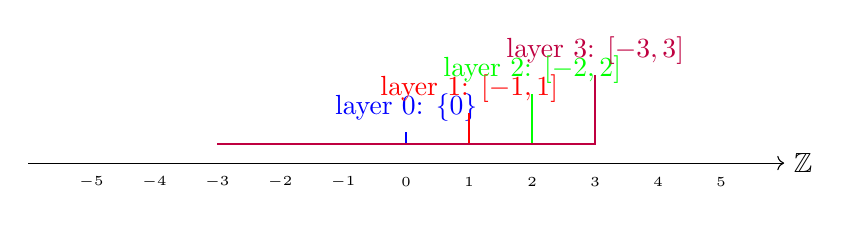
\begin{tikzpicture}[scale=0.8]
\draw[->] (-6,0) -- (6,0) node[right] {$\mathbb{Z}$};
\foreach \x in {-5,...,5}
  \node at (\x,-0.3) {\tiny $\x$};

\draw[thick,blue] (0,0.3) -- (0,0.5) node[above] {layer 0: $\{0\}$};
\draw[thick,red] (-1,0.3) -- (1,0.3) -- (1,0.8) node[above] {layer 1: $[-1,1]$};
\draw[thick,green] (-2,0.3) -- (2,0.3) -- (2,1.1) node[above] {layer 2: $[-2,2]$};
\draw[thick,purple] (-3,0.3) -- (3,0.3) -- (3,1.4) node[above] {layer 3: $[-3,3]$};
\end{tikzpicture}
\end{center}

\begin{proposition}
整数塔 \texttt{intAbsTower} は構造塔の公理をすべて満たす。
特に、倍加写像 $k \mapsto 2k$ は構造塔の準同型を誘導する。
\end{proposition}

\subsection{リスト塔：長さによる階層化}

\begin{definition}[リストの長さ塔]
自然数のリスト $\text{List}\ \mathbb{N}$ 上の構造塔 \texttt{listLengthTower}：
\begin{itemize}
\item $\text{layer}(n) = \{l : \text{List}\ \mathbb{N} \mid |l| \leq n\}$
\item $\text{minLayer}(l) = |l|$
\end{itemize}
\end{definition}

\begin{example}
\begin{align*}
\text{layer}(0) &= \{[]\} \\
\text{layer}(1) &= \{[], [a]\} \\
\text{layer}(2) &= \{[], [a], [a,b]\}
\end{align*}
\end{example}

\subsection{多項式塔：次数による階層化}

\begin{definition}[多項式の次数塔]
有理数係数多項式 $\mathbb{Q}[X]$ 上の構造塔 \texttt{polyDegreeTower}：
\begin{itemize}
\item $\text{layer}(n) = \{p \in \mathbb{Q}[X] \mid \deg(p) \leq n\}$
\item $\text{minLayer}(p) = \deg(p)$
\end{itemize}
\end{definition}

\begin{proposition}
非零スカラー倍 $p \mapsto c \cdot p$ ($c \neq 0$) は構造塔の同型を誘導する。
一方、零写像 $p \mapsto 0$ は等式を保たないが、不等式 $\text{minLayer}(0) \leq \text{minLayer}(p)$ を満たす
$\texttt{HomLe}$ の例を与える。
\end{proposition}

\section{DecidableEvents：有限確率空間と決定可能事象}

\subsection{有限標本空間}

\begin{definition}[有限標本空間]
有限標本空間 $\Omega$ は以下の構造を持つ：
\begin{itemize}
\item 台型 $\Omega.\text{carrier}$ （有限型）
\item $\texttt{Fintype}$ インスタンス（有限性）
\item $\texttt{DecidableEq}$ インスタンス（等号判定可能性）
\end{itemize}
\end{definition}

有限性により、すべての事象の membership が decidable になる。

\subsection{事象と基本演算}

\begin{definition}[事象]
標本空間 $\Omega$ 上の事象は、$\Omega.\text{carrier}$ の部分集合である：
\[
\text{Event}(\Omega) := \text{Set}(\Omega.\text{carrier})
\]
\end{definition}

\begin{definition}[事象の基本演算]
事象 $A, B \subseteq \Omega$ に対して：
\begin{align*}
\emptyset &:= \{\} \quad \text{（空事象）} \\
\Omega &:= \{\omega \mid \omega \in \Omega\} \quad \text{（全事象）} \\
A^c &:= \{\omega \mid \omega \notin A\} \quad \text{（補事象）} \\
A \cup B &:= \{\omega \mid \omega \in A \lor \omega \in B\} \quad \text{（和事象）} \\
A \cap B &:= \{\omega \mid \omega \in A \land \omega \in B\} \quad \text{（積事象）}
\end{align*}
\end{definition}

\begin{theorem}[De Morgan の法則]
任意の事象 $A, B$ に対して：
\begin{align*}
(A \cup B)^c &= A^c \cap B^c \\
(A \cap B)^c &= A^c \cup B^c
\end{align*}
\end{theorem}

\subsection{具体例：サイコロの事象}

\begin{example}[サイコロの標本空間]
$\Omega = \text{Fin}\ 6 = \{0, 1, 2, 3, 4, 5\}$ として、
\begin{align*}
E &= \{\text{偶数}\} = \{0, 2, 4\} \\
O &= E^c = \{1, 3, 5\} \\
B &= \{\text{大きい目}\} = \{3, 4, 5\}
\end{align*}
これらはすべて decidable である。
\end{example}

\section{DecidableAlgebra：有限代数}

\subsection{有限代数の定義}

\begin{definition}[有限代数]
標本空間 $\Omega$ 上の有限代数 $\mathcal{F}$ は、事象の族 $\mathcal{F} \subseteq \mathcal{P}(\Omega)$ であって、
以下を満たすもの：
\begin{enumerate}
\item $\emptyset \in \mathcal{F}$ （空集合を含む）
\item $A \in \mathcal{F} \Rightarrow A^c \in \mathcal{F}$ （補集合で閉じている）
\item $A, B \in \mathcal{F} \Rightarrow A \cup B \in \mathcal{F}$ （和で閉じている）
\end{enumerate}
\end{definition}

\begin{proposition}
有限代数 $\mathcal{F}$ は以下も満たす：
\begin{enumerate}
\item $\Omega \in \mathcal{F}$ （全事象を含む）
\item $A, B \in \mathcal{F} \Rightarrow A \cap B \in \mathcal{F}$ （積で閉じている）
\item $A, B \in \mathcal{F} \Rightarrow A \setminus B \in \mathcal{F}$ （差で閉じている）
\end{enumerate}
\end{proposition}

\subsection{具体的な有限代数}

\begin{example}[自明な代数]
$\mathcal{F}_{\text{trivial}} = \{\emptyset, \Omega\}$ は最小の代数である。
\end{example}

\begin{example}[全体の代数]
$\mathcal{F}_{\text{power}} = \mathcal{P}(\Omega)$ は最大の代数である。
\end{example}

\begin{example}[偶奇代数]
サイコロ空間 $\Omega = \text{Fin}\ 6$ 上で、偶数の目 $E = \{0, 2, 4\}$ から生成される代数は：
\[
\mathcal{F}_{\text{even-odd}} = \{\emptyset, E, E^c, \Omega\}
\]
これは「偶数か奇数か」という情報のみが観測可能な状態を表す。
\end{example}

\begin{center}
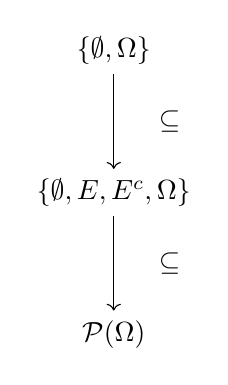
\begin{tikzpicture}[scale=0.9]
\node (trivial) at (0,0) {$\{\emptyset, \Omega\}$};
\node (evenodd) at (0,-2) {$\{\emptyset, E, E^c, \Omega\}$};
\node (power) at (0,-4) {$\mathcal{P}(\Omega)$};

\draw[->] (trivial) -- (evenodd);
\draw[->] (evenodd) -- (power);

\node[right] at (0.5,-1) {$\subseteq$};
\node[right] at (0.5,-3) {$\subseteq$};
\end{tikzpicture}
\end{center}

\subsection{可測関数}

\begin{definition}[可測関数]
関数 $f : \Omega \to \Omega'$ が代数 $(\mathcal{F}, \mathcal{G})$ に関して可測であるとは、
\[
\forall B \in \mathcal{G}, \quad f^{-1}(B) \in \mathcal{F}
\]
が成り立つことをいう。
\end{definition}

可測関数は「観測可能な情報を保存する関数」の形式化である。

\section{DecidableFiltration：離散フィルトレーション}

\subsection{フィルトレーションの定義}

\begin{definition}[離散フィルトレーション]
有限標本空間 $\Omega$ 上の離散フィルトレーション $\mathcal{F}$ は以下のデータからなる：
\begin{itemize}
\item 時間の終端 $N \in \mathbb{N}$ （timeHorizon）
\item 各時刻 $t \leq N$ に対する有限代数 $\mathcal{F}_t$
\item 単調性：$s \leq t \Rightarrow \mathcal{F}_s \subseteq \mathcal{F}_t$
\end{itemize}
\end{definition}

\begin{center}
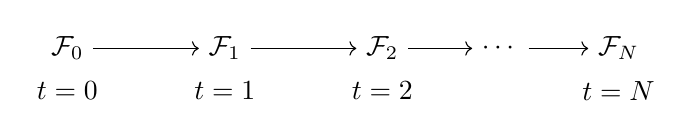
\begin{tikzpicture}
\node (F0) at (0,0) {$\mathcal{F}_0$};
\node (F1) at (2,0) {$\mathcal{F}_1$};
\node (F2) at (4,0) {$\mathcal{F}_2$};
\node (dots) at (5.5,0) {$\cdots$};
\node (FN) at (7,0) {$\mathcal{F}_N$};

\draw[->] (F0) -- (F1);
\draw[->] (F1) -- (F2);
\draw[->] (F2) -- (dots);
\draw[->] (dots) -- (FN);

\node[below] at (0,-0.3) {$t=0$};
\node[below] at (2,-0.3) {$t=1$};
\node[below] at (4,-0.3) {$t=2$};
\node[below] at (7,-0.3) {$t=N$};
\end{tikzpicture}
\end{center}

フィルトレーションは「時間とともに増加する情報」を表現する。

\subsection{構造塔との対応}

\begin{theorem}[フィルトレーションは構造塔]
離散フィルトレーション $\mathcal{F}$ は構造塔のインスタンスである：
\begin{itemize}
\item $\text{carrier} = \text{Event}(\Omega)$ （事象の全体）
\item $\text{Index} = \{0, 1, \ldots, N\}$ （時刻）
\item $\text{layer}(t) = \mathcal{F}_t$ （時刻 $t$ で可観測な事象族）
\item $\text{minLayer}(A) = \min\{t \mid A \in \mathcal{F}_t\}$ （初めて可観測になる時刻）
\end{itemize}
\end{theorem}

この対応により、確率論の概念（フィルトレーション、停止時間）が
構造塔理論の言葉で統一的に扱える。

\subsection{具体例：2段階フィルトレーション}

\begin{example}
時間終端 $N = 1$ として、
\[
\mathcal{F}_0 = \{\emptyset, \Omega\}, \quad \mathcal{F}_1 = \mathcal{P}(\Omega)
\]
とすると、$\mathcal{F}_0 \subseteq \mathcal{F}_1$ が成り立ち、
フィルトレーションをなす。
\end{example}

\section{ComputableStoppingTime：計算可能停止時間}

\subsection{停止時間の定義}

\begin{definition}[停止時間]
フィルトレーション $\mathcal{F}$ に関する停止時間 $\tau$ とは、
写像 $\tau : \Omega \to \mathbb{N}$ であって、
\[
\forall t \leq N, \quad \{\omega \mid \tau(\omega) \leq t\} \in \mathcal{F}_t
\]
を満たすものをいう。
\end{definition}

この条件は「時刻 $t$ までに停止したかどうか」が時刻 $t$ の情報で判定できることを意味する。

\subsection{停止時間の演算}

\begin{proposition}[停止時間の min と max]
$\tau_1, \tau_2$ が停止時間ならば、
\begin{align*}
\min(\tau_1, \tau_2)(\omega) &:= \min(\tau_1(\omega), \tau_2(\omega)) \\
\max(\tau_1, \tau_2)(\omega) &:= \max(\tau_1(\omega), \tau_2(\omega))
\end{align*}
もまた停止時間である。
\end{proposition}

\begin{proof}
$\min$ の場合：
\begin{align*}
\{\min(\tau_1, \tau_2) \leq t\} &= \{\tau_1 \leq t\} \cup \{\tau_2 \leq t\} \in \mathcal{F}_t
\end{align*}

$\max$ の場合：
\begin{align*}
\{\max(\tau_1, \tau_2) \leq t\} &= \{\tau_1 \leq t\} \cap \{\tau_2 \leq t\} \in \mathcal{F}_t
\end{align*}
\end{proof}

\subsection{有界停止時間}

\begin{definition}[有界停止時間]
停止時間 $\tau$ が上界 $N$ で有界であるとは、
\[
\forall \omega, \quad \tau(\omega) \leq N
\]
が成り立つことをいう。
\end{definition}

有界性は Optional Stopping Theorem の重要な仮定である。

\section{AlgorithmicMartingaleCore：確率測度とマルチンゲール}

\subsection{確率質量関数}

\begin{definition}[確率質量関数]
有限標本空間 $\Omega$ 上の確率質量関数 (PMF) $P$ は、写像 $P : \Omega \to \mathbb{Q}$ であって、
\begin{enumerate}
\item $\forall \omega, P(\omega) \geq 0$ （非負性）
\item $\sum_{\omega \in \Omega} P(\omega) = 1$ （全確率 1）
\end{enumerate}
を満たすもの。
\end{definition}

\subsection{期待値}

\begin{definition}[期待値]
ランダム変数 $X : \Omega \to \mathbb{Q}$ の期待値は、
\[
\mathbb{E}_P[X] := \sum_{\omega \in \Omega} P(\omega) \cdot X(\omega)
\]
で定義される。
\end{definition}

\begin{proposition}[期待値の性質]
\begin{enumerate}
\item 定数の期待値：$\mathbb{E}_P[c] = c$
\item 線形性：$\mathbb{E}_P[aX + bY] = a\mathbb{E}_P[X] + b\mathbb{E}_P[Y]$
\item 指示関数：$\mathbb{E}_P[1_A] = P(A)$
\end{enumerate}
\end{proposition}

\subsection{マルチンゲール}

\begin{definition}[離散時間過程]
離散時間過程 $M$ は、写像 $M : \mathbb{N} \times \Omega \to \mathbb{Q}$ である。
時刻 $n$ における値を $M_n$ と書く。
\end{definition}

\begin{definition}[マルチンゲール（簡略版）]
過程 $M$ がフィルトレーション $\mathcal{F}$ に関してマルチンゲールであるとは、
\[
\forall n < N, \quad \mathbb{E}_P[M_{n+1}] = \mathbb{E}_P[M_n]
\]
が成り立つことをいう。
\end{definition}

\begin{definition}[マルチンゲール（強版）]
過程 $M$ が強マルチンゲールであるとは、
任意の $A \in \mathcal{F}_n$ に対して、
\[
\mathbb{E}_P[M_{n+1} \cdot 1_A] = \mathbb{E}_P[M_n \cdot 1_A]
\]
が成り立つことをいう。
\end{definition}

強版の定義は、古典的な条件付き期待値による定義
$\mathbb{E}[M_{n+1} \mid \mathcal{F}_n] = M_n$
の離散有限版に相当する。

\begin{example}[定数過程]
$M_n(\omega) \equiv c$ なる定数過程はマルチンゲールである。
実際、$\mathbb{E}_P[M_n] = c$ がすべての $n$ で成り立つ。
\end{example}

\section{AlgorithmicMartingale\_v0：Optional Stopping Theorem}

\subsection{停止過程}

\begin{definition}[停止過程]
停止時間 $\tau$ による停止過程 $M^\tau$ は、
\[
M^\tau_n(\omega) := M_{\min(n, \tau(\omega))}(\omega)
\]
で定義される。
\end{definition}

\begin{center}
\begin{tikzpicture}[scale=0.9]
\draw[->] (0,0) -- (8,0) node[right] {$n$};
\draw[->] (0,0) -- (0,4) node[above] {$M_n(\omega)$};

\draw[thick,blue] (0,1) -- (1,1.5) -- (2,2) -- (3,2.2) -- (4,2.5) -- (5,3) -- (6,2.8) -- (7,3.2);
\draw[thick,red] (0,1) -- (1,1.5) -- (2,2) -- (3,2.2) -- (3,2.2) -- (4,2.2) -- (5,2.2) -- (6,2.2) -- (7,2.2);

\draw[dashed] (3,0) -- (3,2.2);
\node[below] at (3,0) {$\tau(\omega)$};

\node[blue,right] at (7,3.2) {$M$};
\node[red,right] at (7,2.2) {$M^\tau$};
\end{tikzpicture}
\end{center}

\subsection{Optional Stopping Theorem}

\begin{theorem}[OST：グローバル版]
$M$ が強マルチンゲールで、$\tau$ が有界停止時間 $(\tau \leq N)$ ならば、
\[
\mathbb{E}_P[M_\tau] = \mathbb{E}_P[M_0]
\]
が成り立つ。ここで $M_\tau(\omega) := M_{\tau(\omega)}(\omega)$ である。
\end{theorem}

\subsection{証明の概略}

証明は以下の手順で行う：

\textbf{Step 1: パスごとの分解}

任意の $\omega$ に対して、
\[
M_{\tau(\omega)}(\omega) - M_0(\omega) = \sum_{n=0}^{N-1} (M_{n+1}(\omega) - M_n(\omega)) \cdot 1_{\{\tau(\omega) > n\}}
\]
が成り立つ（テレスコーピング）。

\textbf{Step 2: 期待値への持ち上げ}

期待値を取ると、
\[
\mathbb{E}[M_\tau - M_0] = \sum_{n=0}^{N-1} \mathbb{E}[(M_{n+1} - M_n) \cdot 1_{\{\tau > n\}}]
\]

\textbf{Step 3: 各増分の期待値が 0}

$A_n := \{\tau > n\} = \{\tau \leq n\}^c$ とおくと、$A_n \in \mathcal{F}_n$ である。
強マルチンゲール条件より、
\[
\mathbb{E}[M_{n+1} \cdot 1_{A_n}] = \mathbb{E}[M_n \cdot 1_{A_n}]
\]
したがって、
\[
\mathbb{E}[(M_{n+1} - M_n) \cdot 1_{A_n}] = 0
\]

\textbf{Step 4: 結論}

\[
\mathbb{E}[M_\tau - M_0] = \sum_{n=0}^{N-1} 0 = 0
\]
したがって $\mathbb{E}[M_\tau] = \mathbb{E}[M_0]$ を得る。

\subsection{詳細な証明}

\begin{lemma}[増分の期待値]
強マルチンゲール $M$ と停止時間 $\tau$ に対して、
\[
\mathbb{E}_P[(M_{n+1} - M_n) \cdot 1_{\{\tau > n\}}] = 0
\]
\end{lemma}

\begin{proof}
$A := \{\tau > n\}$ とおく。$\{\tau \leq n\} \in \mathcal{F}_n$ より、
その補集合 $A = \{\tau > n\}$ も $\mathcal{F}_n$ に属する。

強マルチンゲール条件より、
\[
\mathbb{E}_P[M_{n+1} \cdot 1_A] = \mathbb{E}_P[M_n \cdot 1_A]
\]

したがって、
\begin{align*}
\mathbb{E}_P[(M_{n+1} - M_n) \cdot 1_A]
&= \mathbb{E}_P[M_{n+1} \cdot 1_A] - \mathbb{E}_P[M_n \cdot 1_A] \\
&= 0
\end{align*}
\end{proof}

\begin{lemma}[パスごとの増分分解]
任意の $\omega \in \Omega$ に対して、
\[
M_{\tau(\omega)}(\omega) - M_0(\omega) = \sum_{n=0}^{N-1} (M_{n+1}(\omega) - M_n(\omega)) \cdot 1_{\{\tau(\omega) > n\}}
\]
\end{lemma}

\begin{proof}
$k := \tau(\omega)$ とおく。指示関数により、和は $n < k$ の項のみ生き残る：
\begin{align*}
\sum_{n=0}^{N-1} (M_{n+1}(\omega) - M_n(\omega)) \cdot 1_{\{k > n\}}
&= \sum_{n=0}^{k-1} (M_{n+1}(\omega) - M_n(\omega)) \\
&= M_k(\omega) - M_0(\omega)
\end{align*}
最後の等式はテレスコーピングによる。
\end{proof}

\begin{proof}[Optional Stopping Theorem の証明]
パスごとの分解式に期待値を適用すると、
\begin{align*}
\mathbb{E}_P[M_\tau - M_0]
&= \mathbb{E}_P\left[\sum_{n=0}^{N-1} (M_{n+1} - M_n) \cdot 1_{\{\tau > n\}}\right] \\
&= \sum_{n=0}^{N-1} \mathbb{E}_P[(M_{n+1} - M_n) \cdot 1_{\{\tau > n\}}] \quad \text{（有限和と期待値の交換）} \\
&= \sum_{n=0}^{N-1} 0 \quad \text{（Lemma より）} \\
&= 0
\end{align*}

したがって、
\[
\mathbb{E}_P[M_\tau] = \mathbb{E}_P[M_0]
\]
\end{proof}

\subsection{系：和の形の OST}

\begin{corollary}[OST：和形式]
強マルチンゲール $M$ と有界停止時間 $\tau$ に対して、
\[
\sum_{n=0}^{N} \mathbb{E}_P[M_n \cdot 1_{\{\tau = n\}}] = \sum_{n=0}^{N} \mathbb{E}_P[M_0 \cdot 1_{\{\tau = n\}}]
\]
\end{corollary}

\begin{proof}
まず、
\[
M_\tau(\omega) = \sum_{n=0}^{N} M_n(\omega) \cdot 1_{\{\tau(\omega) = n\}}
\]
が成り立つ（各 $\omega$ について丁度一つの $n$ で指示関数が 1）。

期待値を取ると、
\[
\mathbb{E}_P[M_\tau] = \sum_{n=0}^{N} \mathbb{E}_P[M_n \cdot 1_{\{\tau = n\}}]
\]

同様に、
\[
\mathbb{E}_P[M_0] = \sum_{n=0}^{N} \mathbb{E}_P[M_0 \cdot 1_{\{\tau = n\}}]
\]

OST より $\mathbb{E}_P[M_\tau] = \mathbb{E}_P[M_0]$ だから、結論を得る。
\end{proof}

\section{結論と展望}

\subsection{主要な成果}

本論文では、離散有限標本空間上の確率論を構造塔理論の枠組みで統一的に扱う形式化を完成させた：

\begin{enumerate}
\item 構造塔の計算可能な例（整数、リスト、多項式等）の提示
\item 有限標本空間と決定可能事象の定義
\item 有限代数（$\sigma$-代数の離散版）の構築
\item 離散フィルトレーションの構造塔としての定式化
\item 計算可能停止時間の理論
\item Optional Stopping Theorem の完全な形式的証明
\end{enumerate}

すべての定義と証明は Lean 4 で形式化され、計算可能性が保証されている。

\subsection{構造塔理論との統一}

本研究の最も重要な貢献は、DecidableFiltration が構造塔の自然なインスタンスであることを示したことである：

\begin{center}
\begin{tikzpicture}[node distance=3cm]
\node (ST) {構造塔理論};
\node (DF) [below of=ST] {DecidableFiltration};
\node (Prob) [below of=DF] {離散確率論};

\draw[<->] (ST) -- node[right] {インスタンス化} (DF);
\draw[->] (DF) -- node[right] {応用} (Prob);

\node[left] at (-2,-1.5) {minLayer $\leftrightarrow$ 初めて可観測};
\node[left] at (-2,-3) {layer $\leftrightarrow$ 時刻の代数};
\node[left] at (-2,-4.5) {monotone $\leftrightarrow$ 情報増加};
\end{tikzpicture}
\end{center}

\subsection{今後の課題}

\begin{enumerate}
\item \textbf{条件付き期待値の完全な定式化}：現在の強マルチンゲール条件を、
より一般的な $\mathbb{E}[M_{n+1} \mid \mathcal{F}_n] = M_n$ の形式に拡張する。

\item \textbf{無限時間への拡張}：有限時間 $N$ の制約を外し、
無限時間フィルトレーションを扱えるようにする。

\item \textbf{連続時間への拡張}：離散時間から連続時間への一般化。

\item \textbf{他の確率論的定理の形式化}：Doob の不等式、収束定理、
確率微分方程式など。

\item \textbf{構造塔の圏論的性質}：ホモロジー、コホモロジーなどの
高次構造への拡張。
\end{enumerate}

\section*{謝辞}

本論文の Lean コードは Codex (OpenAI) によって生成され、
数学的解説は Claude Code (Anthropic) によって執筆された。
両システムの協力により、形式化と数学的洞察の統合が実現した。

\begin{thebibliography}{99}
\bibitem{williams}
D. Williams,
\textit{Probability with Martingales},
Cambridge University Press, 1991.

\bibitem{grimmett}
G. Grimmett and D. Stirzaker,
\textit{Probability and Random Processes},
Oxford University Press, 2001.

\bibitem{billingsley}
P. Billingsley,
\textit{Probability and Measure},
Wiley, 1995.

\bibitem{kallenberg}
O. Kallenberg,
\textit{Foundations of Modern Probability},
Springer, 2002.

\bibitem{lean4}
The Lean Community,
\textit{The Lean 4 Theorem Prover},
\url{https://lean-lang.org/}, 2024.

\bibitem{mathlib4}
The mathlib Community,
\textit{The Lean Mathematical Library},
\url{https://github.com/leanprover-community/mathlib4}, 2024.

\end{thebibliography}

\appendix

\section{Lean コードの構造}

本論文で扱った理論は、以下のファイル構造で実装されている：

\begin{verbatim}
DecidableStructureTower_Examples.md
  ├─ intAbsTower (整数塔)
  ├─ listLengthTower (リスト塔)
  ├─ finsetCardTower (有限集合塔)
  ├─ polyDegreeTower (多項式塔)
  └─ stringLengthTower (文字列塔)

DecidableEvents.md
  ├─ FiniteSampleSpace
  ├─ Event
  └─ 基本演算 (∅, Ω, A^c, A∪B, A∩B)

DecidableAlgebra.md
  ├─ FiniteAlgebra
  ├─ trivial, powerSet, evenOddAlgebra
  └─ MeasurableFunction

DecidableFiltration.md
  ├─ DecidableFiltration
  ├─ StoppingTime
  └─ min, max 演算

ComputableStoppingTime.md
  ├─ ComputableStoppingTime
  ├─ isBounded
  └─ 具体例

AlgorithmicMartingaleCore.md
  ├─ ProbabilityMassFunction
  ├─ expected
  ├─ SimpleProcess
  └─ IsMartingale

AlgorithmicMartingale_v0.md
  ├─ IsMartingaleStrong
  ├─ stopped process
  ├─ increment_zero
  └─ optionalStopping_theorem
\end{verbatim}

\section{記号表}

\begin{tabular}{ll}
\hline
記号 & 意味 \\
\hline
$\Omega$ & 標本空間 \\
$\mathcal{F}$ & 有限代数 \\
$\mathcal{F}_t$ & 時刻 $t$ の代数 \\
$P$ & 確率質量関数 \\
$\mathbb{E}_P[X]$ & 期待値 \\
$M$ & 離散時間過程 \\
$\tau$ & 停止時間 \\
$M^\tau$ & 停止過程 \\
$N$ & 時間の終端 \\
$1_A$ & 事象 $A$ の指示関数 \\
\hline
\end{tabular}

\end{document}
